\section{Introduction}
\label{sec:introduction}



\par In these laboratory assignement the objective is to study the reaction of an RC circuit under different conditions. From a constant voltage that passes through it, where it works as an open circuit. Up to a sinusoidal voltage, where a detailed study of the node voltages at the capacitor terminals was made as a function of time and frequency. In order to analyze it, we will use different techniques such as Thevenin and Phasor analysis. Then we compare the theoretical and simulation results.

\par The circuit in question is depicted in Figure~\ref{fig:circuit} 


\par In Section~\ref{sec:analysis}, a theoretical analysis of the circuit, using GNU Octave,  is presented. In Section~\ref{sec:simulation}, the circuit is simulated, and the results are compared 
aforementioned one. The conclusions of the study are presented in the last section of the document.

 \FloatBarrier 
 \begin{center}
\begin{figure}
  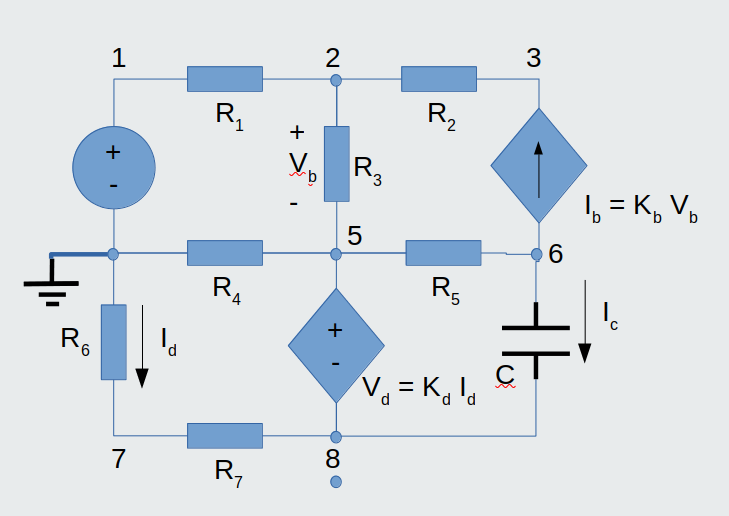
\includegraphics[width=\linewidth]{circuit.png}
  \caption{The circuit with the mesh currents represented by circular arrows}
  \label{fig:circuit}
\end{figure}
\end{center}
\FloatBarrier
